\documentclass[
  11pt,
  letterpaper,
   addpoints,
   answers
  ]{exam}

% Carga el preámbulo localizado en la carpeta superior
\NeedsTeXFormat{LaTeX2e}[2023/04/30]

% Provide the name of your page, the date it was last updated, and a comment about what it's used for
\ProvidesPackage{../exercise-preamble}[2023/04/30 Prof. Cassanelli custom LaTeX style]

% \usepackage{printlen}
% \uselengthunit{in}\printlength{\textwidth}

% PACKAGES
\usepackage[dvipsnames]{xcolor}

\usepackage{graphicx}
\graphicspath{{../figures}}
\usepackage{amsmath,amsthm,amssymb,mathtools,mathrsfs}
\usepackage{commath}
\usepackage{upgreek}
\usepackage{cancel}
\usepackage{enumerate}
\usepackage[font=small]{caption}
\usepackage[normalem]{ulem}
\usepackage{steinmetz}
\usepackage{enumitem}
\usepackage[left=1.5cm, right=1.5cm, top=1cm]{geometry}
\usepackage{wrapfig}

% REFERENCES AND OTHERS
\usepackage{../aas_macros}
\usepackage{natbib}
\bibpunct{(}{)}{;}{a}{}{,}

\usepackage{tikz}
\usepackage{tikz-3dplot}
\usepackage{circuitikz}
\usepackage{pgfplots}
\pgfplotsset{compat=1.15}
\usepgfplotslibrary{smithchart}
\usetikzlibrary{
  decorations.pathmorphing,
  decorations.markings,
  calc,
  patterns,
  decorations,
  angles,
  quotes,
  ext.topaths.arcthrough,
  shapes
  }

\usepackage{siunitx}
\sisetup{
    range-phrase=\text{--},
    range-units=single,
    separate-uncertainty=true,
    print-unity-mantissa=false
    }
\DeclareSIUnit{\gauss}{G}
\DeclareSIUnit{\jansky}{Jy}

\newcommand{\iu}{\mathrm{i}\mkern1mu}
\newcommand{\ju}{\mathrm{j}\mkern1mu}
\newcommand{\euler}{\mathrm{e}}
\newcommand{\exponential}[1]{\mathrm{exp}\left[#1\right]}
\newcommand{\uvec}[1]{\widehat{\mathbf{#1}}}
\newcommand{\uvecs}[1]{\boldsymbol{\widehat{#1}}}
\newcommand{\bvec}[1]{\boldsymbol{\mathcal{#1}}}

\usepackage{hyperref}
\hypersetup{
    % bookmarks=true,
    unicode=true,
    pdftoolbar=true,
    pdfmenubar=true,
    pdffitwindow=false,
    pdfstartview={FitH},
    pdftitle={EL3103},
    pdfauthor={Tomas Cassanelli},
    pdfcreator={Tomas Cassanelli},
    pdfnewwindow=true,
    colorlinks=true,
    linkcolor=Violet,
    citecolor=Violet,
    urlcolor=Violet
    }

% Exam document class
\renewcommand{\figurename}{Figura}
\renewcommand{\tablename}{Cuadro}
\pagestyle{empty}

\usepackage[spanish]{cleveref}

\crefname{question}{\protect{pregunta}}{\protect{preguntas}}
\Crefname{question}{\protect{Pregunta}}{\protect{Preguntas}}
\creflabelformat{question}{#2{#1}#3}

\renewcommand{\solutiontitle}{\noindent\textbf{Solución:}\par\noindent}
\bracketedpoints
\pointname{~puntos}

\endinput

% Paquetes locales
\usepackage{float}
\usepackage{booktabs} % para \toprule, \midrule, \bottomrule
\usepackage{xcolor} % para colores

% Macros locales
\newcommand{\Rel}{\mathfrak{R}} % símbolo para la reluctancia

\begin{document}

\noindent
\begin{minipage}{0.47\textwidth}

\includegraphics[width=\textwidth]{../fcfm_die}
\end{minipage}
\begin{minipage}{0.53\textwidth}
\begin{center}
\large\textbf{Análisis de Sistemas Dinámicos y Estimación} (EL3204-1) \\
\large\textbf{Ejercicio 1} \\
\normalsize Prof.~ Marcos Orchard - Sebastián Espinosa.\\
\normalsize Prof.~Aux.~Erik Sáez
\end{center}
\end{minipage}

\vspace{0.5cm}
\noindent\fbox{%
  \parbox{\dimexpr\linewidth-2\fboxsep-2\fboxrule\relax}{%
    	\textbf{Instrucciones:} La tarea se puede realizar en grupos de 3 con un plazo máximo hasta el viernes 17 de Octubre; no se aceptarán atrasos. El formato deberá ser entregada escrita a mano o en tablet (letra legible), además de entrega virtual de los códigos que utilicen.
  }%
}

\vspace{.85cm}

    %%%%%%%%%%%%%%%%%%%%%%%%%%%
    Considere el sistema electromecánico de la figura~\ref{fig:relay}, que modela de forma simplificada el funcionamiento de un relé electromagnético utilizado en el sistema de control de un robot industrial para el ensamblaje de componentes electrónicos de precisión. Este dispositivo consta de un núcleo de hierro de sección transversal $A$ en el cual se induce flujo magnético mediante una bobina de $N$ vueltas. El relé controla actuadores neumáticos que operan las pinzas del robot, donde la precisión y eficiencia energética son críticas para la operación. Para este estudio, usted podrá modificar el voltaje de excitación $e(t)$ y analizará cómo el entrehierco modula la inductancia $L(x)$, la fuerza de atracción magnética y la dinámica de conmutación del sistema.\\

    \noindent\fbox{\parbox{0.92\linewidth}{\textbf{Nota:} Considere que el movimiento de la armadura móvil ocurre únicamente en una dirección (sobre el eje $x$), es decir, el desplazamiento es unidimensional.}}

\begin{figure}[h!]
  \centering
  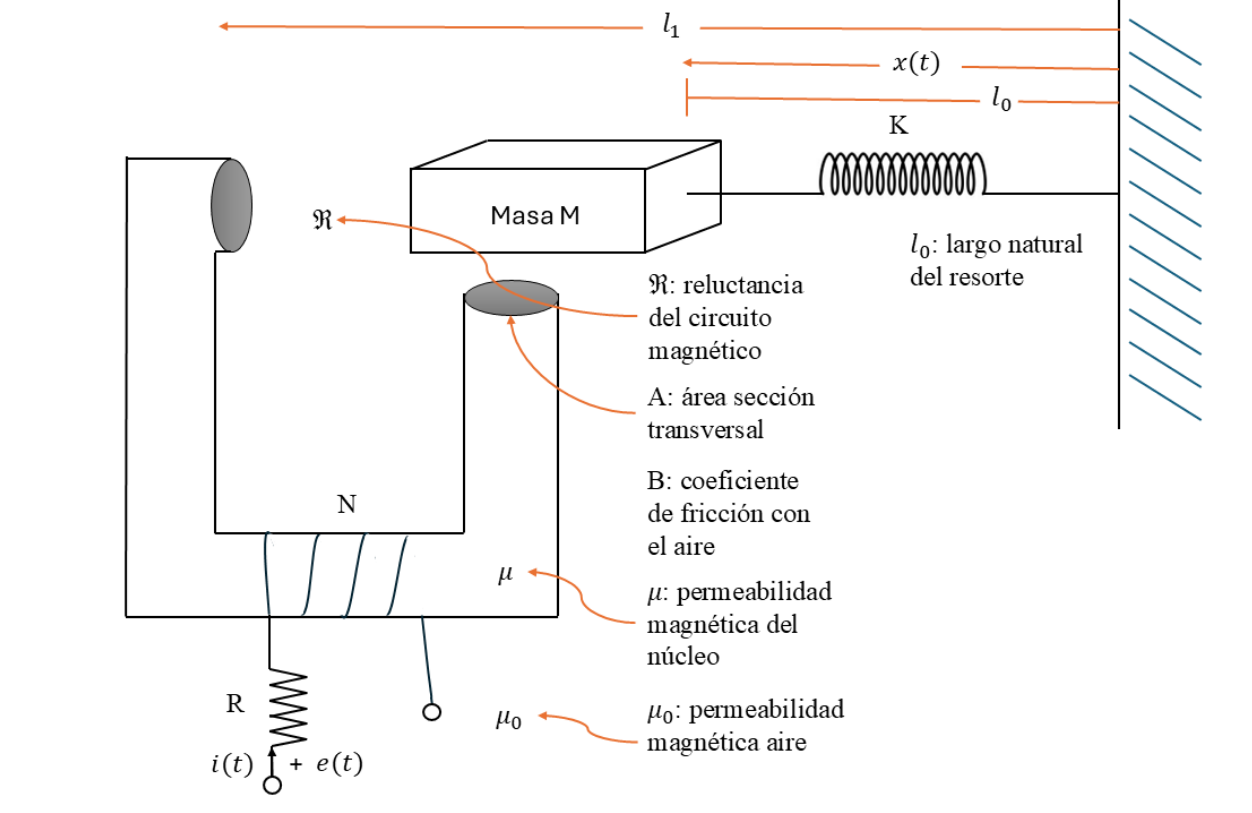
\includegraphics[width=0.8\textwidth,keepaspectratio]{Ejercicio_1_1}
  \caption{Sistema electromecánico del relé electromagnético mostrando la armadura móvil de masa $M$, el resorte de constante $K$, el entrehierro variable $x(t)$, y el circuito eléctrico equivalente con resistencia $R$ y voltaje de excitación $e(t)$.}
  \label{fig:relay}
\end{figure}

Los parámetros del sistema, junto con sus respectivas unidades de medida, se detallan en la Tabla~\ref{tab:variables}.

\begin{table}[H]
  \centering
  \caption{Variables y parámetros del sistema}
  \label{tab:variables}
  \small
  \begin{tabular}{@{}c p{9.5cm} c@{}}
    \toprule
    \textbf{Variable/Parámetro} & \textbf{Definición} & \textbf{Unidad} \\
    \midrule
    $x(t)$      & Posición de la armadura móvil entre $l_0$ y $l_1$ & m \\
    $i(t)$      & Corriente por la bobina                           & A \\
    $L(x)$      & Inductancia de la bobina                          & H \\
  $\Rel$      & Reluctancia del circuito magnético                & A/Wb (1/H) \\
    $e(t)$      & Voltaje en la bobina                              & V \\
    $M$         & Masa de la pieza                                  & kg \\
    $K$         & Coeficiente de rigidez del resorte                & N/m \\
    $B$         & Coeficiente de fricción viscosa del aire          & N/(m/s) \\
    $R$         & Resistencia eléctrica de la bobina                & $\Omega$ \\
    $A$         & Área de la sección transversal del núcleo         & m$^2$ \\
    $\mu$       & Permeabilidad magnética del núcleo                & H/m \\
    $\mu_0$     & Permeabilidad magnética del aire                  & H/m \\
    $N$         & Número de espiras de la bobina                    & -- \\
    \bottomrule
  \end{tabular}
\end{table}

Para el análisis electromagnético del sistema, es fundamental comprender la distribución del flujo magnético y las reluctancias involucradas. La fuerza magnetomotriz generada por la bobina está dada por $F_m = N \cdot i(t)$. Aplicando la ley de Ampère para un circuito magnético cerrado, se establece que:
\begin{align}
  N \cdot i = H_n \cdot l_n + H_g \cdot l_g  = \frac{B_n}{\mu} \cdot l_n + \frac{B_g}{\mu_0} \cdot l_g .
\end{align}
donde $B_n$ y $l_n$ corresponden a la densidad de flujo magnético y la longitud promedio del camino en el núcleo de hierro, respectivamente. Por otra parte, $B_g$ y $l_g$ representan la densidad de flujo magnético en el entrehierro y su longitud. La geometría del núcleo magnético se ilustra detalladamente en la Figura~\ref{fig:core}.

\begin{figure}[h!]
  \centering
  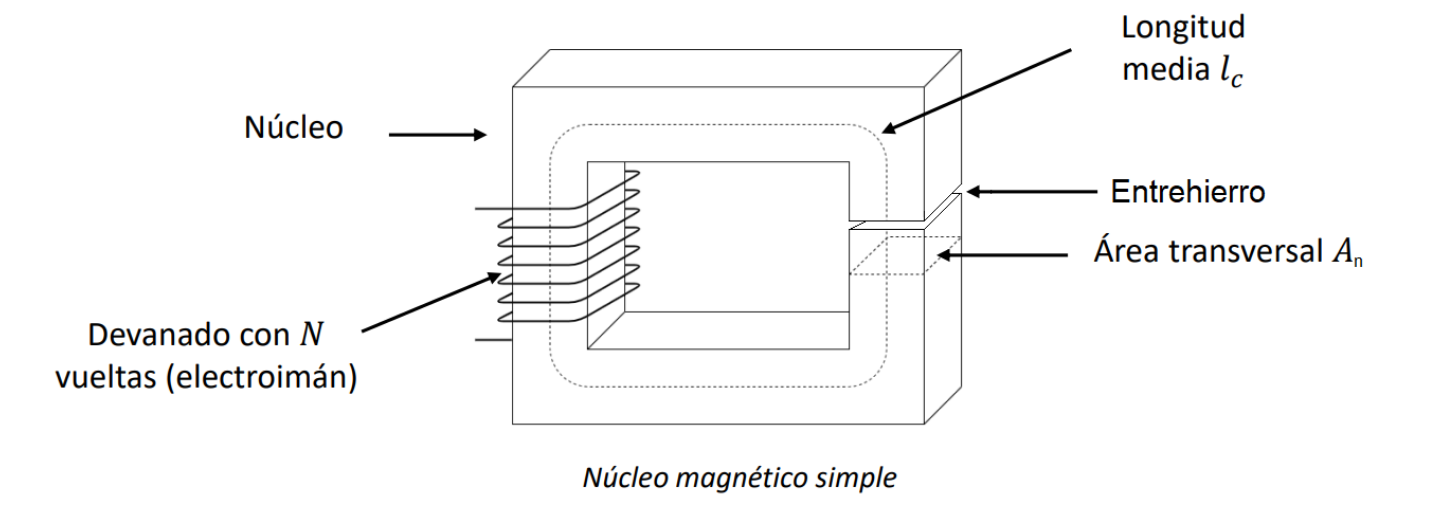
\includegraphics[width=0.85\textwidth,keepaspectratio]{Ejercicio_1_2}
  \caption{Diagrama del núcleo magnético simple mostrando el devanado de $N$ vueltas, el núcleo de hierro con longitud media $l_c$, el entrehierro de longitud variable, y el área transversal $A_n$ del flujo magnético.}
  \label{fig:core}
\end{figure}

El flujo magnético se define como la integral del campo magnético sobre la superficie transversal:
\begin{align}
  \int B_{n,g}\, \mathrm{d}s = \phi.
\end{align}
Considerando que el campo magnético es uniforme en la sección transversal del núcleo, se obtiene:
\begin{align}
  B_{n,g} = \frac{\phi}{A_n}.
\end{align}
Sustituyendo esta expresión en la ecuación de Ampère:
\begin{align}
  N \cdot i = \frac{\phi}{A_n \mu} \cdot l_n + \frac{\phi}{A_n \mu_0} \cdot l_g = \phi\!\left(\frac{l_n}{A_n \mu} + \frac{l_g}{A_n \mu_0}\right).
\end{align}

La reluctancia $\Rel$ es un parámetro fundamental que cuantifica la resistencia de un material al flujo magnético. Esta magnitud depende de la permeabilidad del material magnético ($\mu$), el área de la sección transversal ($A$) y la longitud del camino magnético ($l$):
\begin{align}
  \Rel = \frac{l}{A\,\mu}.
\end{align}
Aplicando este concepto al circuito magnético del relé:
\begin{align}
  N\,i &= \phi\,(\Rel_n + \Rel_g), \\
  \phi &= \frac{N\,i}{\Rel_n + \Rel_g}.
\end{align}

La relación entre el voltaje de la bobina y las variables electromagnéticas se establece mediante las ecuaciones fundamentales del electromagnetismo:
\begin{align}
  V_{\text{bobina}} = L\,\frac{\mathrm{d}i}{\mathrm{d}t} = N\,\frac{\mathrm{d}\phi}{\mathrm{d}t}.
\end{align}
Integrando esta ecuación con respecto al tiempo:
\begin{align}
  L\,i = N\,\phi.
\end{align}
Combinando con la expresión del flujo magnético:
\begin{align}
  L\,i = N\, \frac{N\, i}{\Rel_n + \Rel_g}
\end{align}
Definiendo la reluctancia total como $\Rel_{\text{total}} = \Rel_n + \Rel_g$ y despejando la inductancia:
\begin{align}
  L = \frac{N^2}{\Rel}
\end{align}

En el sistema analizado coexisten dos tipos principales de reluctancia: la reluctancia del entrehierro (debido al aire) y la reluctancia del núcleo de hierro. Dado que el hierro presenta una permeabilidad magnética mucho mayor que el aire, su reluctancia es considerablemente menor. Esta aproximación permite simplificar el análisis considerando que tanto el núcleo fijo como la armadura móvil están fabricados en hierro. El objetivo del estudio es analizar la dinámica del movimiento de la armadura de masa $M$ y la corriente del sistema, respondiendo a las preguntas formuladas en las siguientes secciones.
\newpage
\hrulefill
\begin{center}
\textbf{Valores numéricos de los parámetros del sistema}
\end{center}

\begin{table}[h!]
  \centering
  \caption{Parámetros numéricos del sistema electromecánico del relé electromagnético utilizados para el análisis cuantitativo, simulaciones y diseño del observador. Estos valores representan configuraciones típicas encontradas en aplicaciones industriales de precisión.}
  \label{tab:parametros-numericos}
  \begin{tabular}{@{}c c@{}}
    \toprule
    \textbf{Parámetro} & \textbf{Valor} \\
    \midrule
    $l_1$ & $0.03\,[\mathrm{m}]$ \\
    $l_0$ & $0.02\,[\mathrm{m}]$ \\
    $N$   & $200$ espiras \\
    $a$   & $0.0001\,[\mathrm{m}^2]$ \\
    $\mu_0$ & $4\pi \times 10^{-7}\,[\mathrm{H/m}]$ \\
    $K$   & $0.01\,[\mathrm{N/m}]$ \\
    $B$   & $0.00000001\,[\mathrm{N/(m/s)}]$ \\
    \bottomrule
  \end{tabular}
\end{table}
\begin{questions}
\question \textbf{Modelamiento matemático}
\begin{enumerate}
  \item \textcolor{blue}{\textbf{[0.15 pts]}} Establezca de forma clara todas las hipótesis simplificatorias del sistema. Considere que la Figura~\ref{fig:core} no tiene errores y, por tanto, si considera que falta algún dato o parámetro indique cómo abordará esto para que el modelo tenga sentido. Además, se aconseja investigar sobre transformadores ideales.

  \item \textcolor{blue}{\textbf{[0.3 pts]}} Formule el modelo matemático. Para ello deberá encontrar dos ecuaciones; una para la parte eléctrica del sistema y la otra para la parte mecánica del mismo. \emph{Hint}: la fuerza magnética interactúa con la pieza móvil según $F_m = \frac{1}{2} i^2\, \frac{\mathrm{d}L}{\mathrm{d}x}$. Además, si el valor $L$ de una inductancia varía con el tiempo a través de una función $g(t)$, entonces, el voltaje en esa inductancia será $V_{\text{ind}} = \frac{\mathrm{d}}{\mathrm{d}t}\left[L(g(t)) \cdot i(t)\right]$.

  \item \textcolor{blue}{\textbf{[0.25 pts]}} En base al contexto del problema, indique las variables que corresponden a la/s entrada/s, salida/s y variable/s de estado del sistema. Replantee el modelo como un sistema matricial de la forma $\dot{\vec{X}}(t) = \vec{F}\big(\vec{X}(t), u(t)\big)$ con su respectiva salida $\vec{Y}(t) = C \cdot \vec{X}(t)$, donde $\vec{X}(t)$ representa el vector de estados, $C$ la matriz de salida y $u(t)$ la/s entrada/s al sistema.

  \item \textcolor{blue}{\textbf{[0.15 pts]}} Encuentre el/los estado/s de equilibrio del sistema no lineal.

  \item \textcolor{blue}{\textbf{[0.15 pts]}} Encuentre las ecuaciones del/los punto/s de operación que asegura que la pieza móvil esté en una posición arbitraria $x_0$. Luego, exprese una única ecuación que involucre la posición de la pieza móvil y la entrada $u_0(t)$ (no es necesario despejar la posición de la pieza móvil).
\end{enumerate}

\question \textbf{Linealización-Laplace-MTE}

\begin{enumerate}
  \item \textcolor{blue}{\textbf{[0.3 pts]}} Linealice el sistema planteado en la pregunta anterior en torno a un punto de operación arbitrario $(\vec{X}(t_0), u(t_0))$ con tal de obtener la expresión $\dot{\vec{X}} = A \cdot \vec{X} + B \cdot u$, donde $A$ es la matriz de estado y $B$ la matriz de entrada.

  \item \textcolor{blue}{\textbf{[0.2 pts]}} Considere el sistema linealizado del primer punto. Evalúe el sistema en torno al estado de equilibrio que usted considere pertinente según lo que encontró en P1.4. \textbf{Importante:} Para las siguientes preguntas se considerará este sistema en particular.

  \item \textcolor{blue}{\textbf{[0.25 pts]}} Obtenga la MTE del sistema linealizado en torno al punto de equilibrio.

  \item \textcolor{blue}{\textbf{[0.25 pts]}} Obtenga la función de transferencia del sistema linealizado en torno al punto de equilibrio.
\end{enumerate}

\question \textbf{Determinación de estados}
\begin{enumerate}
  \item \textcolor{blue}{\textbf{[0.5 pts]}} Encuentre los estados cero del sistema linealizado alrededor del punto de equilibrio. Especifique claramente la definición usada y calcule los vectores de estado que satisfacen la condición de salida nula.

  \item \textcolor{blue}{\textbf{[0.5 pts]}} Encuentre los estados "tierra" (estados de reposo) del sistema linealizado alrededor del punto de equilibrio. Indique las condiciones iniciales asociadas si corresponde.
\end{enumerate}

\question \textbf{Polos, respuesta al impulso, RESC y RENC}
\begin{enumerate}
  \item \textcolor{blue}{\textbf{[0.2 pts]}} Determine los polos del sistema linealizado en torno al punto de equilibrio y comente su implicancia dinámica (estabilidad, oscilación, amortiguamiento).

  \item \textcolor{blue}{\textbf{[0.2 pts]}} Usando la función de transferencia del sistema linealizado, obtenga la respuesta al impulso en el dominio del tiempo y describa sus características principales.

  \item \textcolor{blue}{\textbf{[0.2 pts]}} Calcule la respuesta en estado cero (RESC) para el sistema linealizado en torno al punto de equilibrio ante una entrada arbitraria. Explique las hipótesis usadas.

  \item \textcolor{blue}{\textbf{[0.2 pts]}} Calcule la respuesta en estado (RENC) para condiciones iniciales arbitrarias del sistema linealizado. Presente la expresión en términos de la exponencial matricial si procede.

  \item \textcolor{blue}{\textbf{[0.2 pts]}} Exprese la solución completa del sistema linealizado alrededor del punto de equilibrio combinando RESC y RENC (solución general).
\end{enumerate}

\question \textbf{Estabilidad, controlabilidad y observabilidad}
\begin{enumerate}
  \item \textcolor{blue}{\textbf{[0.2 pts]}} Determine la estabilidad del sistema linealizado en torno al punto de equilibrio. Explique el criterio utilizado (por ejemplo, ubicación de polos o matriz $A$).

  \item \textcolor{blue}{\textbf{[0.3 pts]}} Determine si el sistema es controlable. Justifique mediante el criterio de Kalman (matriz de controlabilidad) o argumento equivalente.

  \item \textcolor{blue}{\textbf{[0.2 pts]}} Considere ahora que $C = [111]$. Determine si el sistema es observable.

  \item \textcolor{blue}{\textbf{[0.3 pts]}} Considere ahora que $C = [111]$. Diseñe un observador de Luenberger para el sistema a tiempo continuo. Como criterio de diseño, para elegir los polos del observador, considere que los polos del observador deben ser, al menos, 3 veces más negativos que todos los polos del sistema original. Puede dejar expresadas las ecuaciones (3) para resolver el problema (no es necesario que lo resuelva).
\end{enumerate}

\question \textbf{Simulaciones Matlab}

\begin{enumerate}
  \item \textcolor{blue}{\textbf{[0.3 pts]}} Considere el contexto de la parte 5 de la pregunta 1. Grafique en un mismo gráfico las fuerzas eléctrica y mecánica en función de la posición $x(t)$ de la pieza móvil entre el rango $[l_0, l_1]$ (con el paso que usted estime pertinente). Indique la posición y corriente que asegura equilibrio en el sistema considerando que el voltaje es $e(t)) = 2~[\text{V}]$. Para ello considere los siguientes casos de la Tabla~\ref{tab:casos-corriente}:

  \begingroup
  \renewcommand{\tablename}{Tabla}
  \begin{table}[H]
    \centering
    \caption{Valores de corriente constante para el análisis de equilibrio del sistema electromecánico. Estos casos permiten evaluar el comportamiento de las fuerzas magnética y mecánica en función de la posición de la armadura móvil bajo diferentes condiciones de operación del relé electromagnético.}
    \label{tab:casos-corriente}
    \small
    \begin{tabular}{|c|c|}
      \hline
      \textbf{Caso} & $I_0$ [A] \\
      \hline
      a & 1 \\
      \hline
      b & 2 \\
      \hline
      c & 3 \\
      \hline
    \end{tabular}
  \end{table}
  \endgroup

  \item \textcolor{blue}{\textbf{[0.4 pts]}} Simule el sistema y analice la respuesta completa del sistema de tiempo continuo frente a un escalón unitario y señales sinusoidales con 2 frecuencias distintas, considerando al menos dos condiciones iniciales en todos los casos. Las frecuencias de las señales sinusoidales y las componentes que definen condiciones iniciales deben generarse mediante realizaciones de variables aleatorias con distribución uniforme, cuyo soporte debe ser debidamente reportado. Analice sus resultados y concluya cómo afectan las condiciones iniciales y las diferentes entradas al sistema.

  \item \textcolor{blue}{\textbf{[0.3 pts]}} Implemente el observador anteriormente diseñado, y simule el sistema observado para entradas y condiciones iniciales generados bajo el mismo criterio que la pregunta anterior. Debe graficar el error en el observador para cada uno de los estados, además de las salidas del sistema original y del sistema observado. Comente sobre sus resultados.
\end{enumerate}
\end{questions}
\hrulefill
\newpage
\begin{solution}
  \subsection*{\textcolor{blue}{[0.15 Ptos]} Resolución 1.1}

    Para el modelamiento del sistema electromecánico del relé electromagnético, es necesario establecer las siguientes hipótesis simplificatorias organizadas por categorías:

    \subsubsection*{Hipótesis Electromagnéticas:}
    \begin{enumerate}
      \item \textbf{Núcleo de hierro ideal}: La permeabilidad magnética del hierro es muy alta ($\mu \gg \mu_0$), por lo que la reluctancia del núcleo de hierro es despreciable comparada con la del entrehierro. Esto permite considerar $\Rel_{\text{total}} \approx \Rel_{\text{entrehierro}}$.
      \item \textbf{Campo magnético uniforme}: El flujo magnético se distribuye uniformemente en la sección transversal $A$ del núcleo, permitiendo usar $B = \phi/A$.
      \item \textbf{No saturación magnética}: El material del núcleo opera en la región lineal de la curva B-H, manteniendo la permeabilidad constante.
      \item \textbf{Flujo de dispersión despreciable}: Todo el flujo magnético se confina al núcleo y entrehierro, sin fugas significativas.
    \end{enumerate}

    \subsubsection*{Hipótesis Mecánicas:}
    \begin{enumerate}
      \item \textbf{Movimiento unidimensional}: La armadura móvil se desplaza únicamente en la dirección del eje $x$ (horizontal), sin rotaciones ni desplazamientos laterales.
      \item \textbf{Masa puntual}: La masa $M$ de la armadura móvil es constante e invariante en el tiempo.
      \item \textbf{Resorte ideal}: El resorte cumple la ley de Hooke con constante elástica $K$ invariante, masa despreciable, y operación en régimen lineal.
      \item \textbf{Fricción viscosa lineal}: El amortiguamiento del aire sigue la ley $F_r = B\dot{x}$ con coeficiente $B$ constante.
      \item \textbf{Gravedad despreciable}: Los efectos gravitacionales son insignificantes comparados con las fuerzas electromagnéticas y elásticas del sistema.
    \end{enumerate}

    \subsubsection*{Hipótesis Eléctricas:}
    \begin{enumerate}
      \item \textbf{Resistencia óhmica ideal}: La resistencia $R$ de la bobina es constante y cumple la ley de Ohm.
      \item \textbf{Capacitancia despreciable}: Los efectos capacitivos parásitos del sistema son insignificantes.
      \item \textbf{Propiedades magnéticas constantes}: Las permeabilidades $\mu$ y $\mu_0$ son invariantes en el tiempo y temperatura.
    \end{enumerate}

    \textbf{Parámetro faltante identificado}: Del análisis de la Figura~\ref{fig:core}, se requiere especificar el área de sección transversal $A$. Según la Tabla de parámetros numéricos, se utilizará $A = a = 0.0001\,[\mathrm{m}^2]$.
    \subsection*{\textcolor{blue}{[0.3 Ptos]} Resolución 1.2}
    
    El sistema electromecánico del relé requiere el análisis de dos subsistemas acoplados: el mecánico y el eléctrico. A continuación se desarrollan ambas ecuaciones.

    \subsubsection*{Análisis Mecánico - Segunda Ley de Newton}
    
    Las fuerzas que actúan sobre la armadura móvil de masa $M$ son:
    \begin{itemize}
        \item $F_m$: Fuerza magnética de atracción (hacia el núcleo fijo)
        \item $F_E$: Fuerza elástica del resorte (restauradora)
        \item $F_r$: Fuerza de fricción viscosa del aire (opuesta al movimiento)
    \end{itemize}

    Aplicando la segunda ley de Newton en la dirección $x$:
    \begin{align}
        M \ddot{x}(t) = F_m - F_E - F_r
    \end{align}

    \textbf{Fuerza magnética}: Utilizando la expresión proporcionada en el hint, la fuerza magnética de atracción es:
    \begin{align}
        F_m = \frac{1}{2} i^2(t) \frac{\partial L(x)}{\partial x}
    \end{align}

    \textbf{Fuerza elástica}: Considerando que el resorte tiene longitud natural cuando $x = l_0$:
    \begin{align}
        F_E = K(x(t) - l_0)
    \end{align}

    \textbf{Fuerza de fricción viscosa}:
    \begin{align}
        F_r = B \dot{x}(t)
    \end{align}

    \subsubsection*{Deducción de la Inductancia Variable}
    
    La inductancia del sistema depende de la reluctancia total del circuito magnético:
    \begin{align}
        L(x) = \frac{N^2}{\Rel_{\text{total}}}
    \end{align}

    Donde la reluctancia total es la suma de las reluctancias del núcleo y del entrehierro:
    \begin{align}
        \Rel_{\text{total}} = \Rel_{\text{núcleo}} + \Rel_{\text{entrehierro}}
    \end{align}

    Bajo la hipótesis de núcleo de hierro ideal ($\Rel_{\text{núcleo}} \ll \Rel_{\text{entrehierro}}$):
    \begin{align}
        \Rel_{\text{total}} &\approx \Rel_{\text{entrehierro}} = \frac{l_{\text{entrehierro}}}{A \mu_0}
    \end{align}

    De la geometría del sistema, la longitud del entrehierro es:
    \begin{align}
        l_{\text{entrehierro}} = l_1 - x(t)
    \end{align}

    Por lo tanto, la inductancia variable es:
    \begin{align}
        L(x(t)) = \frac{N^2 A \mu_0}{l_1 - x(t)}
    \end{align}

    Calculando la derivada parcial necesaria para la fuerza magnética:
    \begin{align}
        \frac{\partial L(x)}{\partial x} = \frac{\partial}{\partial x}\left(\frac{N^2 A \mu_0}{l_1 - x(t)}\right) = \frac{N^2 A \mu_0}{(l_1 - x(t))^2}
    \end{align}

    \textbf{Ecuación mecánica completa}:
    \begin{align}
        \boxed{M \ddot{x}(t) = \frac{1}{2} i^2(t) \frac{N^2 A \mu_0}{(l_1 - x(t))^2} - K(x(t) - l_0) - B \dot{x}(t)}
    \end{align}

    \subsubsection*{Análisis Eléctrico - Ley de Kirchhoff de Voltajes (KVL)}
    
    Aplicando KVL al circuito eléctrico:
    \begin{align}
        e(t) = R i(t) + V_{\text{bobina}}
    \end{align}

    La tensión en la bobina corresponde a la derivada temporal del flujo enlazado. Dado que tanto la inductancia como la corriente varían con el tiempo:
    \begin{align}
        V_{\text{bobina}} &= \frac{d}{dt}[L(x(t)) \cdot i(t)]\\
        &= \frac{\partial L(x)}{\partial x} \frac{dx}{dt} i(t) + L(x(t)) \frac{di(t)}{dt}
    \end{align}

    Sustituyendo las expresiones conocidas:
    \begin{align}
        V_{\text{bobina}} = i(t) \frac{N^2 A \mu_0}{(l_1 - x(t))^2} \dot{x}(t) + \frac{N^2 A \mu_0}{l_1 - x(t)} \dot{i}(t)
    \end{align}

    \textbf{Ecuación eléctrica completa}:
    \begin{align}
        \boxed{e(t) = R i(t) + i(t) \frac{N^2 A \mu_0}{(l_1 - x(t))^2} \dot{x}(t) + \frac{N^2 A \mu_0}{l_1 - x(t)} \dot{i}(t)}
    \end{align}

    Estas dos ecuaciones no lineales acopladas describen completamente la dinámica del sistema electromecánico del relé.
\subsection*{\textcolor{blue}{[0.25 Ptos]} Resolución 1.3}

El análisis de variables de entrada, salida y estado es fundamental para representar el sistema electromecánico en forma de espacio de estados.

\subsubsection*{Identificación de Variables}

\textbf{Variable de entrada}: El voltaje aplicado a la bobina constituye la entrada del sistema:
\[
u(t) = e(t)
\]

\textbf{Variables de estado}: Para un sistema de orden 3, se requieren 3 variables de estado que capturen toda la información dinámica del sistema. Se eligen:
\[
\vec{X}(t) = \begin{bmatrix}
x_1(t) \\ x_2(t) \\ x_3(t)
\end{bmatrix} = \begin{bmatrix}
x(t) \\ \dot{x}(t) \\ i(t)
\end{bmatrix}
\]

Donde:
\begin{itemize}
    \item $x_1(t) = x(t)$: Posición de la armadura móvil
    \item $x_2(t) = \dot{x}(t)$: Velocidad de la armadura móvil  
    \item $x_3(t) = i(t)$: Corriente en la bobina
\end{itemize}

\textbf{Variables de salida}: Se considera que todas las variables de estado son medibles:
\[
\vec{Y}(t) = \begin{bmatrix}
x(t) \\ \dot{x}(t) \\ i(t)
\end{bmatrix}, \qquad
C = \begin{bmatrix}
1 & 0 & 0 \\
0 & 1 & 0 \\
0 & 0 & 1
\end{bmatrix} = I_3
\]

\subsubsection*{Representación en Espacio de Estados}

A partir de las ecuaciones derivadas en la sección 1.2, se obtiene:

\textbf{Ecuaciones de estado}:
\begin{align}
\dot{x}_1(t) &= x_2(t) \\
\dot{x}_2(t) &= \frac{1}{2M} x_3^2(t) \frac{N^2 A \mu_0}{(l_1 - x_1(t))^2} - \frac{K}{M}(x_1(t) - l_0) - \frac{B}{M} x_2(t) \\
\dot{x}_3(t) &= \frac{u(t)(l_1 - x_1(t))}{N^2 A \mu_0} - \frac{R x_3(t)(l_1 - x_1(t))}{N^2 A \mu_0} - \frac{x_3(t) x_2(t)}{l_1 - x_1(t)}
\end{align}

\textbf{Forma matricial compacta}:
\begin{align}
\dot{\vec{X}}(t) &= \vec{F}(\vec{X}(t), u(t)) = \begin{bmatrix}
x_2(t) \\[4pt]
\displaystyle \frac{1}{2M} x_3^2(t) \frac{N^2 A \mu_0}{(l_1 - x_1(t))^2} - \frac{K}{M}(x_1(t) - l_0) - \frac{B}{M} x_2(t) \\[8pt]
\displaystyle \frac{u(t)(l_1 - x_1(t))}{N^2 A \mu_0} - \frac{R x_3(t)(l_1 - x_1(t))}{N^2 A \mu_0} - \frac{x_3(t) x_2(t)}{l_1 - x_1(t)}
\end{bmatrix}
\end{align}

\textbf{Ecuación de salida}:
\begin{align}
\vec{Y}(t) = C \vec{X}(t) = I_3 \vec{X}(t)
\end{align}

\subsubsection*{Características del Modelo}

\textbf{No linealidad}: El sistema presenta no linealidades debido a:
\begin{itemize}
    \item Término cuadrático $x_3^2(t)$ en la fuerza magnética
    \item Producto cruzado $x_3(t) x_2(t)$ en la ecuación eléctrica
    \item Términos recíprocos $(l_1 - x_1(t))^{-1}$ y $(l_1 - x_1(t))^{-2}$
\end{itemize}

\textbf{Acoplamiento}: Existe fuerte acoplamiento bidireccional entre los subsistemas mecánico y eléctrico, donde:
\begin{itemize}
    \item La corriente $i(t)$ genera fuerza magnética que afecta la dinámica mecánica
    \item El movimiento $\dot{x}(t)$ induce voltaje que afecta la dinámica eléctrica
\end{itemize}

\textbf{Dominio de validez}: El modelo es válido para $l_0 \leq x(t) \leq l_1$ para evitar singularidades en las expresiones.
\subsection*{\textcolor{blue}{[0.15 Ptos]} Resolución 1.4}

Para encontrar los estados de equilibrio del sistema no lineal, se debe establecer la condición $\dot{\vec{X}}(t) = \vec{0}$ con entrada constante $u(t) = e(t) = 0$. En equilibrio, todas las derivadas temporales de las variables de estado son cero, lo que implica:
\begin{align}
\dot{x}_1 &= 0 \quad \Rightarrow \quad x_2 = 0 \\
\dot{x}_2 &= 0 \\
\dot{x}_3 &= 0
\end{align}

De la primera condición se obtiene directamente que $x_2 = \dot{x} = 0$, es decir, la velocidad de la armadura móvil debe ser nula en equilibrio. Para analizar la tercera ecuación, consideramos que $\dot{i} = 0$ con entrada nula $u = e(t) = 0$:
\begin{align}
\frac{0 \cdot (l_1 - x_1)}{N^2 A \mu_0} - \frac{R x_3 (l_1 - x_1)}{N^2 A \mu_0} - \frac{x_3 \cdot 0}{l_1 - x_1} &= 0\\
-\frac{R x_3 (l_1 - x_1)}{N^2 A \mu_0} &= 0
\end{align}

Dado que $R > 0$, $N^2 A \mu_0 > 0$, y $(l_1 - x_1) > 0$ para $x_1 < l_1$, la única solución posible es $x_3 = i(t) = 0$. Esto significa que en equilibrio no circula corriente por la bobina.

Finalmente, analizando la segunda ecuación con las condiciones ya encontradas ($i = 0$ y $\dot{x} = 0$):
\begin{align}
\frac{1}{2M} \cdot 0^2 \cdot \frac{N^2 A \mu_0}{(l_1 - x_1)^2} - \frac{K}{M}(x_1 - l_0) - \frac{B}{M} \cdot 0 &= 0\\
-\frac{K}{M}(x_1 - l_0) &= 0\\
x_1 - l_0 &= 0
\end{align}

Por lo tanto, $x_1 = x(t) = l_0$, indicando que la armadura móvil se posiciona en la longitud natural del resorte. El único estado de equilibrio del sistema no lineal con entrada nula es:
\begin{align}
\boxed{\vec{X}_{eq} = \begin{bmatrix}
l_0 \\
0 \\
0
\end{bmatrix}}
\end{align}

Este resultado tiene perfecto sentido físico: sin voltaje aplicado, la armadura móvil se posiciona en $x = l_0$ donde el resorte no ejerce fuerza elástica, no hay movimiento ($\dot{x} = 0$), y no circula corriente ($i = 0$) ya que no hay excitación eléctrica. Sin corriente, no existe fuerza magnética, por lo que el sistema se equilibra naturalmente en la posición de reposo del resorte.

\subsection*{\textcolor{blue}{[0.15 Ptos]} Resolución 1.5}

Para encontrar los puntos de operación que aseguran que la pieza móvil esté en una posición arbitraria $x_0$, debemos considerar el equilibrio del sistema con entrada constante no nula. En este caso, el vector de estados de operación es:
\begin{align}
\vec{X}_p = \begin{bmatrix}
x_0 \\
\dot{x} \\
i_0
\end{bmatrix} = \begin{bmatrix}
x_0 \\
0 \\
i_0
\end{bmatrix}
\end{align}

donde $\dot{x} = 0$ en equilibrio y $i_0$ es la corriente de operación que mantiene la posición deseada $x_0$.

Las ecuaciones de equilibrio se obtienen haciendo $\dot{\vec{X}} = \vec{0}$. De la primera ecuación, confirmamos que $\dot{x} = 0$ en equilibrio. De la segunda ecuación, el balance de fuerzas mecánicas requiere:
\begin{align}
\frac{1}{2M} i_0^2 \frac{N^2 A \mu_0}{(l_1 - x_0)^2} - \frac{K}{M}(x_0 - l_0) - \frac{B}{M} \cdot 0 = 0
\end{align}

Simplificando y despejando la corriente de operación:
\begin{align}
\frac{1}{2M} i_0^2 \frac{N^2 A \mu_0}{(l_1 - x_0)^2} &= \frac{K}{M}(x_0 - l_0)\\
i_0^2 &= \frac{2K(x_0 - l_0)(l_1 - x_0)^2}{N^2 A \mu_0}
\end{align}

Para que exista solución real, se requiere que $(x_0 - l_0) \geq 0$, es decir, $x_0 \geq l_0$. Esto tiene sentido físico ya que se necesita una fuerza magnética atractiva para mantener la armadura en una posición donde el resorte esté comprimido. La corriente de operación resulta:
\begin{align}
i_{0,1} = +\sqrt{\frac{2K(x_0 - l_0)(l_1 - x_0)^2}{N^2 A \mu_0}}, \quad i_{0,2} = -\sqrt{\frac{2K(x_0 - l_0)(l_1 - x_0)^2}{N^2 A \mu_0}}
\end{align}

Esto indica que tenemos dos puntos de operación posibles para cada posición $x_0 > l_0$, correspondientes a corrientes de signos opuestos.

Para encontrar la relación entre la posición $x_0$ y la entrada de operación $u_0 = e(t)$, analizamos la tercera ecuación de equilibrio con $\dot{x} = 0$ e $\dot{i} = 0$:
\begin{align}
\frac{e(t)(l_1 - x_0)}{N^2 A \mu_0} - \frac{R i_0 (l_1 - x_0)}{N^2 A \mu_0} - \frac{i_0 \cdot 0}{l_1 - x_0} = 0
\end{align}

Simplificando:
\begin{align}
e(t)(l_1 - x_0) = R i_0 (l_1 - x_0)
\end{align}

Como $(l_1 - x_0) \neq 0$ para $x_0 < l_1$, obtenemos:
\begin{align}
e(t) = R i_0
\end{align}

Sustituyendo la expresión de $i_0$:
\begin{align}
\boxed{e(t) = R \sqrt{\frac{2K(x_0 - l_0)(l_1 - x_0)^2}{N^2 A \mu_0}}}
\end{align}

Esta ecuación establece la relación única entre la posición deseada $x_0$ y la entrada requerida $u_0 = e(t)$. Para la solución con corriente positiva, el voltaje debe ser positivo, mientras que para la solución con corriente negativa, el voltaje debe ser negativo. El sistema requiere mayor voltaje para posiciones más alejadas de $l_0$ debido al incremento en la fuerza elástica del resorte que debe ser equilibrada por la fuerza magnética.

\subsection*{\textcolor{blue}{[0.3 Ptos]} Resolución 2.1}

Para linealizar el sistema no lineal en torno a un punto de operación arbitrario $(\vec{X}(t_0), u(t_0))$, utilizamos la aproximación de Taylor de primer orden. El sistema linealizado se expresa como $\dot{\tilde{X}} = A \tilde{X} + B \tilde{u}$, donde $\tilde{X} = \vec{X} - \vec{X}(t_0)$ y $\tilde{u} = u - u(t_0)$ representan las desviaciones respecto al punto de operación.

Partiendo del sistema no lineal original:
\begin{align}
\dot{\vec{X}} = \vec{F}(\vec{X}, u) = \begin{bmatrix}
x_2 \\[4pt]
\displaystyle \frac{1}{2M} x_3^2 \frac{N^2 A \mu_0}{(l_1 - x_1)^2} - \frac{K}{M}(x_1 - l_0) - \frac{B}{M} x_2 \\[8pt]
\displaystyle \frac{u(l_1 - x_1)}{N^2 A \mu_0} - \frac{R x_3 (l_1 - x_1)}{N^2 A \mu_0} - \frac{x_3 x_2}{l_1 - x_1}
\end{bmatrix}
\end{align}

La aproximación lineal se obtiene mediante $\dot{\tilde{X}} \approx \frac{\partial \vec{F}}{\partial \vec{X}}\Big|_{(\vec{X}(t_0), u(t_0))} \tilde{X} + \frac{\partial \vec{F}}{\partial u}\Big|_{(\vec{X}(t_0), u(t_0))} \tilde{u}$.

Calculamos las matrices jacobianas $A = \frac{\partial \vec{F}}{\partial \vec{X}}$ y $B = \frac{\partial \vec{F}}{\partial u}$. Para la matriz de estado, las derivadas parciales de cada componente de $\vec{F}$ son:

De $f_1 = x_2$:
\begin{align}
\frac{\partial f_1}{\partial x_1} = 0, \quad \frac{\partial f_1}{\partial x_2} = 1, \quad \frac{\partial f_1}{\partial x_3} = 0
\end{align}

De $f_2 = \frac{1}{2M} x_3^2 \frac{N^2 A \mu_0}{(l_1 - x_1)^2} - \frac{K}{M}(x_1 - l_0) - \frac{B}{M} x_2$:
\begin{align}
\frac{\partial f_2}{\partial x_1} &= \frac{1}{M} x_3^2 \frac{N^2 A \mu_0}{(l_1 - x_1)^3} - \frac{K}{M}\\
\frac{\partial f_2}{\partial x_2} &= -\frac{B}{M}\\
\frac{\partial f_2}{\partial x_3} &= \frac{1}{M} x_3 \frac{N^2 A \mu_0}{(l_1 - x_1)^2}
\end{align}

De $f_3 = \frac{u(l_1 - x_1)}{N^2 A \mu_0} - \frac{R x_3 (l_1 - x_1)}{N^2 A \mu_0} - \frac{x_3 x_2}{l_1 - x_1}$:
\begin{align}
\frac{\partial f_3}{\partial x_1} &= -\frac{u}{N^2 A \mu_0} + \frac{R x_3}{N^2 A \mu_0} + \frac{x_3 x_2}{(l_1 - x_1)^2}\\
\frac{\partial f_3}{\partial x_2} &= -\frac{x_3}{l_1 - x_1}\\
\frac{\partial f_3}{\partial x_3} &= -\frac{R(l_1 - x_1)}{N^2 A \mu_0} - \frac{x_2}{l_1 - x_1}
\end{align}

Para la matriz de entrada:
\begin{align}
\frac{\partial f_1}{\partial u} = 0, \quad \frac{\partial f_2}{\partial u} = 0, \quad \frac{\partial f_3}{\partial u} = \frac{l_1 - x_1}{N^2 A \mu_0}
\end{align}

Por lo tanto, las matrices del sistema linealizado son:
\begin{align}
A = \begin{bmatrix}
0 & 1 & 0 \\[4pt]
\displaystyle \frac{x_3^2 N^2 A \mu_0}{M(l_1 - x_1)^3} - \frac{K}{M} & -\frac{B}{M} & \displaystyle \frac{x_3 N^2 A \mu_0}{M(l_1 - x_1)^2} \\[8pt]
\displaystyle \frac{R x_3 - u}{N^2 A \mu_0} + \frac{x_3 x_2}{(l_1 - x_1)^2} & -\frac{x_3}{l_1 - x_1} & -\frac{R(l_1 - x_1)}{N^2 A \mu_0} - \frac{x_2}{l_1 - x_1}
\end{bmatrix}
\end{align}

\begin{align}
B = \begin{bmatrix}
0 \\
0 \\
\displaystyle \frac{l_1 - x_1}{N^2 A \mu_0}
\end{bmatrix}
\end{align}

Estas matrices deben evaluarse en el punto de operación específico $(\vec{X}(t_0), u(t_0))$ para obtener el sistema linealizado correspondiente. El modelo resultante $\dot{\tilde{X}} = A \tilde{X} + B \tilde{u}$ permite el análisis lineal del comportamiento dinámico del sistema en las cercanías del punto de operación seleccionado.

\subsection*{\textcolor{blue}{[0.2 Ptos]} Resolución 2.2}

Para evaluar el sistema linealizado en torno al estado de equilibrio encontrado en la pregunta 1.4, consideramos el punto de operación con entrada nula $\mu = u = 0$. El estado de equilibrio corresponde a:
\begin{align}
\vec{X}_{eq} = \begin{bmatrix}
x_{eq} \\ \dot{x}_{eq} \\ i_{eq}
\end{bmatrix} = \begin{bmatrix}
l_0 \\ 0 \\ 0
\end{bmatrix}
\end{align}

Evaluando las matrices $A$ y $B$ en este punto de equilibrio $(\vec{X}_{eq}, u_{eq} = 0)$, sustituimos los valores $x_1 = l_0$, $x_2 = 0$, $x_3 = 0$, y $u = 0$ en las expresiones generales obtenidas en la sección anterior.

Los elementos de la matriz de estado $A$ se calculan como sigue. Para la primera fila:
\begin{align}
\frac{\partial f_1}{\partial x_1} = 0, \quad
\frac{\partial f_1}{\partial x_2} = 1, \quad
\frac{\partial f_1}{\partial x_3} = 0
\end{align}

Para la segunda fila, considerando que en equilibrio $x_3 = 0$:
\begin{align}
\frac{\partial f_2}{\partial x_1}\Big|_{eq} &= \frac{1}{M} \cdot 0^2 \cdot \frac{N^2 A \mu_0}{(l_1 - l_0)^3} - \frac{K}{M} = -\frac{K}{M}\\
\frac{\partial f_2}{\partial x_2}\Big|_{eq} &= -\frac{B}{M}\\
\frac{\partial f_2}{\partial x_3}\Big|_{eq} &= \frac{1}{M} \cdot 0 \cdot \frac{N^2 A \mu_0}{(l_1 - l_0)^2} = 0
\end{align}

Para la tercera fila, todos los términos con $x_2$, $x_3$ y $u$ se anulan en equilibrio:
\begin{align}
\frac{\partial f_3}{\partial x_1}\Big|_{eq} &= -\frac{0}{N^2 A \mu_0} + \frac{R \cdot 0}{N^2 A \mu_0} + \frac{0 \cdot 0}{(l_1 - l_0)^2} = 0\\
\frac{\partial f_3}{\partial x_2}\Big|_{eq} &= -\frac{0}{l_1 - l_0} = 0\\
\frac{\partial f_3}{\partial x_3}\Big|_{eq} &= -\frac{R(l_1 - l_0)}{N^2 A \mu_0} - \frac{0}{l_1 - l_0} = -\frac{R(l_1 - l_0)}{N^2 A \mu_0}
\end{align}

La matriz de entrada $B$ evaluada en el punto de equilibrio es:
\begin{align}
B\Big|_{eq} = \begin{bmatrix}
0 \\[2pt] 0 \\[2pt] \displaystyle \frac{l_1 - l_0}{N^2 A \mu_0}
\end{bmatrix}
\end{align}

Reuniendo todos los elementos, el sistema linealizado en torno al punto de equilibrio resulta:
\begin{align}
\boxed{
\dot{\tilde{X}} = \begin{bmatrix}
0 & 1 & 0 \\[6pt]
-\displaystyle\frac{K}{M} & -\displaystyle\frac{B}{M} & 0 \\[6pt]
0 & 0 & -\displaystyle\frac{R(l_1 - l_0)}{N^2 A \mu_0}
\end{bmatrix} \tilde{X} + \begin{bmatrix}
0 \\[2pt] 0 \\[2pt] \displaystyle \frac{l_1 - l_0}{N^2 A \mu_0}
\end{bmatrix} \tilde{u}
}
\end{align}

donde $\tilde{X} = \vec{X} - \vec{X}_{eq}$ y $\tilde{u} = u - u_{eq}$ representan las desviaciones respecto al punto de equilibrio.

Este resultado revela características importantes del sistema linealizado. En primer lugar, se observa un desacoplamiento parcial entre los subsistemas mecánico y eléctrico para pequeñas perturbaciones alrededor del equilibrio. Las primeras dos filas describen la dinámica mecánica como un oscilador masa-resorte-amortiguador clásico de segundo orden, caracterizado por la frecuencia natural $\omega_n = \sqrt{K/M}$ y el coeficiente de amortiguamiento $\zeta = \frac{B}{2\sqrt{KM}}$. 

Por otro lado, la tercera fila representa la dinámica eléctrica como un sistema de primer orden independiente, con constante de tiempo $\tau = \frac{N^2 A \mu_0}{R(l_1 - l_0)}$. Esta separación en el comportamiento lineal facilita significativamente el análisis de estabilidad y el diseño de controladores, ya que cada subsistema puede estudiarse de forma independiente en primera aproximación.

\subsection*{\textcolor{blue}{[0.25 Ptos]} Resolución 2.3}

Para obtener la Matriz de Transición de Estados (MTE), necesitamos calcular $e^{At}$ donde $A$ es la matriz de estado del sistema linealizado. Partiendo de la matriz obtenida en la sección anterior:
\begin{align}
A = \begin{bmatrix}
0 & 1 & 0 \\
-\displaystyle\frac{K}{M} & -\displaystyle\frac{B}{M} & 0 \\
0 & 0 & -\displaystyle\frac{R(l_1 - l_0)}{N^2 A \mu_0}
\end{bmatrix}
\end{align}

Utilizaremos diagonalización para calcular la exponencial matricial. Primero, encontramos los valores propios resolviendo $\det(A - \lambda I) = 0$:
\begin{align}
\det(A - \lambda I) = \begin{vmatrix}
-\lambda & 1 & 0 \\
-\displaystyle\frac{K}{M} & -\displaystyle\frac{B}{M} - \lambda & 0 \\
0 & 0 & -\displaystyle\frac{R(l_1 - l_0)}{N^2 A \mu_0} - \lambda
\end{vmatrix}
\end{align}

Expandiendo por la tercera columna:
\begin{align}
P_A(\lambda) &= -\lambda \cdot \left(-\frac{B}{M} - \lambda\right) \cdot \left(-\frac{R(l_1 - l_0)}{N^2 A \mu_0} - \lambda\right) - 1 \cdot \left(-\frac{K}{M}\right) \cdot \left(-\frac{R(l_1 - l_0)}{N^2 A \mu_0} - \lambda\right)\\
&= -\lambda \left(\frac{B}{M} + \lambda\right)\left(\frac{R(l_1 - l_0)}{N^2 A \mu_0} + \lambda\right) - \frac{K}{M}\left(\frac{R(l_1 - l_0)}{N^2 A \mu_0} + \lambda\right)\\
&= \left(\frac{R(l_1 - l_0)}{N^2 A \mu_0} + \lambda\right)\left[-\lambda\left(\frac{B}{M} + \lambda\right) - \frac{K}{M}\right]\\
&= \left(\frac{R(l_1 - l_0)}{N^2 A \mu_0} + \lambda\right)\left(-\lambda^2 - \frac{B}{M}\lambda - \frac{K}{M}\right) = 0
\end{align}

De este polinomio característico obtenemos:

**Primer valor propio:**
\begin{align}
\lambda_1 = -\frac{R(l_1 - l_0)}{N^2 A \mu_0}
\end{align}

**Segundo y tercer valor propio** (de la ecuación cuadrática):
\begin{align}
\lambda^2 + \frac{B}{M}\lambda + \frac{K}{M} = 0
\end{align}

Aplicando la fórmula cuadrática:
\begin{align}
\lambda_{2,3} = \frac{-\frac{B}{M} \pm \sqrt{\left(\frac{B}{M}\right)^2 - 4\frac{K}{M}}}{2}
\end{align}

Definiendo $\alpha = \frac{B}{2M}$ y $\beta = \frac{1}{2}\sqrt{\left(\frac{B}{M}\right)^2 - 4\frac{K}{M}}$:
\begin{align}
\lambda_2 &= -\frac{B}{2M} + \frac{1}{2}\sqrt{\left(\frac{B}{M}\right)^2 - 4\frac{K}{M}} = -\alpha + \beta\\
\lambda_3 &= -\frac{B}{2M} - \frac{1}{2}\sqrt{\left(\frac{B}{M}\right)^2 - 4\frac{K}{M}} = -\alpha - \beta
\end{align}

Ahora calculamos los vectores propios resolviendo $(A - \lambda_i I)v_i = 0$ para cada valor propio.

**Para $\lambda_1$:**
\begin{align}
(A - \lambda_1 I)v_1 = \begin{bmatrix}
\frac{R(l_1 - l_0)}{N^2 A \mu_0} & 1 & 0 \\
-\frac{K}{M} & -\frac{B}{M} + \frac{R(l_1 - l_0)}{N^2 A \mu_0} & 0 \\
0 & 0 & 0
\end{bmatrix} \begin{bmatrix} x_1 \\ x_2 \\ x_3 \end{bmatrix} = \begin{bmatrix} 0 \\ 0 \\ 0 \end{bmatrix}
\end{align}

De la tercera ecuación: cualquier valor de $x_3$ es válido, elegimos $x_3 = 1$.
De la primera ecuación: $x_2 + \frac{R(l_1 - l_0)}{N^2 A \mu_0} x_1 = 0$, por lo que $x_2 = 0$ y $x_1 = 0$.
Por tanto: $v_1 = [0, 0, 1]^T$.

**Para $\lambda_2 = -\alpha + \beta$:**
\begin{align}
(A - \lambda_2 I)v_2 = \begin{bmatrix}
\alpha - \beta & 1 & 0 \\
-\frac{K}{M} & -\frac{B}{M} + \alpha - \beta & 0 \\
0 & 0 & -\frac{R(l_1 - l_0)}{N^2 A \mu_0} + \alpha - \beta
\end{bmatrix} \begin{bmatrix} x_1 \\ x_2 \\ x_3 \end{bmatrix} = \begin{bmatrix} 0 \\ 0 \\ 0 \end{bmatrix}
\end{align}

De la primera ecuación: $x_2 = (\alpha - \beta)x_1$.
Para evitar la solución trivial, elegimos $x_2 = 1$, entonces $x_1 = \alpha - \beta$.
De la tercera ecuación: $x_3 = 0$.
Por tanto: $v_2 = [\alpha - \beta, 1, 0]^T$.

**Para $\lambda_3 = -\alpha - \beta$:**
Siguiendo un proceso similar:
$v_3 = [\alpha + \beta, 1, 0]^T$.

La matriz modal es:
\begin{align}
P = \begin{bmatrix}
0 & \alpha - \beta & \alpha + \beta \\
0 & 1 & 1 \\
1 & 0 & 0
\end{bmatrix}
\end{align}

Calculamos $P^{-1}$ utilizando la fórmula de la inversa. El determinante de $P$ es:
\begin{align}
\det(P) = 1 \cdot \begin{vmatrix} \alpha - \beta & \alpha + \beta \\ 1 & 1 \end{vmatrix} = (\alpha - \beta) - (\alpha + \beta) = -2\beta
\end{align}

Por tanto:
\begin{align}
P^{-1} = \frac{1}{-2\beta} \begin{bmatrix}
0 & 0 & -2\beta \\
\alpha + \beta & 2\beta & 0 \\
\alpha - \beta & -2\beta & 0
\end{bmatrix} = \begin{bmatrix}
0 & 0 & 1 \\
\frac{\alpha + \beta}{2\beta} & \frac{1}{2\beta} & 0 \\
\frac{\alpha - \beta}{2\beta} & -\frac{1}{2\beta} & 0
\end{bmatrix}
\end{align}

Con $A = PDP^{-1}$ donde $D = \text{diag}(\lambda_1, \lambda_2, \lambda_3)$, la MTE se calcula como:
\begin{align}
e^{At} = P e^{Dt} P^{-1}
\end{align}

donde:
\begin{align}
e^{Dt} = \begin{bmatrix}
e^{\lambda_1 t} & 0 & 0 \\
0 & e^{\lambda_2 t} & 0 \\
0 & 0 & e^{\lambda_3 t}
\end{bmatrix}
\end{align}

Realizando la multiplicación matricial $Pe^{Dt}P^{-1}$:
\begin{align}
e^{At} &= \begin{bmatrix}
0 & \alpha - \beta & \alpha + \beta \\
0 & 1 & 1 \\
1 & 0 & 0
\end{bmatrix} \begin{bmatrix}
e^{\lambda_1 t} & 0 & 0 \\
0 & e^{\lambda_2 t} & 0 \\
0 & 0 & e^{\lambda_3 t}
\end{bmatrix} \begin{bmatrix}
0 & 0 & 1 \\
\frac{\alpha + \beta}{2\beta} & \frac{1}{2\beta} & 0 \\
\frac{\alpha - \beta}{2\beta} & -\frac{1}{2\beta} & 0
\end{bmatrix}
\end{align}

Después de realizar las operaciones matriciales:
\begin{align}
\boxed{
e^{At} = \begin{bmatrix}
\frac{(\alpha-\beta)e^{\lambda_2 t} + (\alpha+\beta)e^{\lambda_3 t}}{2\beta} & \frac{(\alpha^2-\beta^2)(e^{\lambda_2 t} - e^{\lambda_3 t})}{2\beta} & 0 \\[6pt]
\frac{e^{\lambda_2 t} + e^{\lambda_3 t}}{2\beta} & \frac{(\alpha+\beta)e^{\lambda_2 t} + (\alpha-\beta)e^{\lambda_3 t}}{2\beta} & 0 \\[6pt]
0 & 0 & e^{\lambda_1 t}
\end{bmatrix}
}
\end{align}

Esta MTE confirma el desacoplamiento entre los subsistemas mecánico (submatriz $2 \times 2$ superior izquierda) y eléctrico (elemento $(3,3)$). La estructura triangular por bloques facilita el análisis de la respuesta temporal del sistema para cualquier condición inicial mediante $\tilde{X}(t) = e^{At}\tilde{X}(0)$.

\subsection*{\textcolor{blue}{[0.1 Ptos]} Resolución 2.4}

Para obtener la función de transferencia del sistema, comenzamos con la relación matricial:
\begin{align}
H(s) = C(sI - A)^{-1}B
\end{align}

Como $C = I$ (matriz identidad $3 \times 3$), necesitamos calcular $(sI - A)^{-1}$:

\begin{align}
H(s) = \frac{1}{2B} \begin{bmatrix}
\frac{\alpha - B}{s - \lambda_2} & \frac{\alpha + B}{s - \lambda_3} & (x^* - B^*) \cdot \left(\frac{1}{s - \lambda_2} + \frac{1}{s - \lambda_3}\right) & 0 \\
\frac{1}{s - \lambda_2} & \frac{1}{s - \lambda_3} & \alpha + B \cdot \frac{\alpha - B}{s - \lambda_2} & 0 \\
0 & 0 & 0 & \frac{2B}{s - \lambda_1} \\
\end{bmatrix} \begin{bmatrix}
0 \\
0 \\
\frac{l_1 - l_0}{N^2 A \mu_0 (s - \lambda_1)}
\end{bmatrix}
\end{align}

Dado que las 2 primeras filas presentan un 0 al final y el vector $\vec{B}$ tiene 2 ceros al principio, la multiplicación de las 2 primeras filas con $\vec{B}$ resulta 0.

Por lo tanto:
\begin{align}
H(s) = \frac{1}{2B} \begin{bmatrix}
0 \\
0 \\
\frac{l_1 - l_0}{N^2 A \mu_0 (s - \lambda_1)}
\end{bmatrix}
\end{align}

\subsection*{\textcolor{blue}{[0.5 Ptos]} Resolución 3.1}

Para encontrar los estados cero del sistema linealizado, debemos aplicar la definición: un estado cero $\vec{X}_e$ es aquel que satisface que para toda entrada nula, la salida es nula. En otras palabras, si la entrada al sistema es $u(t) = 0$ para todo $t$, entonces la salida $\vec{y}(t) = 0$ para todo $t$.

En nuestro sistema, la relación salida-estado está dada por $\vec{y}(t) = C\vec{X}(t)$, donde la matriz de salida es:
\begin{align}
C = \begin{bmatrix}
1 & 0 & 0 \\
0 & 1 & 0 \\
0 & 0 & 1
\end{bmatrix}_{3 \times 3}
\end{align}

Esto significa que la salida del sistema es exactamente igual al vector de estados:
\begin{align}
\vec{y}(t) = \vec{X}(t) = \begin{bmatrix}
x(t) \\
\dot{x}(t) \\
i(t)
\end{bmatrix}
\end{align}

Dado que requerimos $\vec{y}(t) = \vec{0}$ para todo $t$ cuando la entrada es nula, y como $\vec{y}(t) = \vec{X}(t)$, se deduce que necesariamente $\vec{X}(t) = \vec{0}$ para todo $t$.

Por lo tanto, el único estado cero del sistema es:
\begin{align}
\vec{X}_e = \begin{bmatrix}
x_0 \\
\dot{x}_0 \\
i_0
\end{bmatrix} = \vec{0}
\end{align}

\subsection*{\textcolor{blue}{[0.5 Ptos]} Resolución 3.2}

Los estados "tierra" (o estados de reposo) son aquellos vectores de estado inicial $\vec{X}_T$ que satisfacen que para cualquier estado inicial $\vec{X}_0$, si la entrada es nula, el sistema converge a $\vec{X}_T$. 

En términos matemáticos, para entrada nula $e(t) = 0$, se debe cumplir que:
\begin{align}
\lim_{t \to \infty} \vec{X}(t) = \vec{X}_T
\end{align}

Para analizar este comportamiento, consideremos qué sucede cuando la entrada es nula ($e(t) = 0$). En esta condición, la corriente también se hace nula ($i(t) = 0$), lo que implica que la fuerza magnética es cero:
\begin{align}
\vec{F}_{\text{magnética}} = 0
\end{align}

Sin fuerza magnética actuando sobre el sistema, para una posición inicial $x(t_0)$ dada en la masa, el resorte ejercerá una fuerza y la masa comenzará a oscilar. 

Sin embargo, debido a la presencia de la fuerza de roce viscosa, la masa se detendrá progresivamente cuando llegue al equilibrio mecánico. Este equilibrio se establece cuando la suma de fuerzas sobre la masa es cero.

Las condiciones de equilibrio son:
\begin{itemize}
    \item $x(t_{\infty}) = l_0$ (posición de equilibrio natural del resorte)
    \item $\dot{x}(t_{\infty}) = 0$ (velocidad nula en equilibrio)
    \item $i(t_{\infty}) = 0$ (corriente nula sin entrada eléctrica)
\end{itemize}

Por consiguiente, el estado tierra del sistema es:
\begin{align}
\vec{X}_{\text{TIERRA}} = \begin{bmatrix}
l_0 \\
0 \\
0
\end{bmatrix}
\end{align}

\subsection*{\textcolor{blue}{[0.2 Ptos]} Resolución 4.1}

Para determinar los polos del sistema linealizado, debemos encontrar los valores propios de la matriz de estado $A$. Dado que los polos de la matriz son los mismos que de la función de transferencia, ya que se tiene que $H(s) = C(sI-A)^{-1}B$, los polos corresponden a los valores de $s$ que hacen que $\det(sI-A) = 0$.

Del análisis de la matriz de estado del sistema linealizado en torno al punto de equilibrio, los polos son:

\begin{align}
\lambda_1 &= -\frac{R(l_1-l_0)}{N^2A\mu_0}
\end{align}

\begin{align}
\lambda_2 &= -\frac{B}{2M} + \frac{1}{2}\sqrt{\frac{B^2}{M^2} - 4\frac{K}{M}}
\end{align}

\begin{align}
\lambda_3 &= -\frac{B}{2M} - \frac{1}{2}\sqrt{\frac{B^2}{M^2} - 4\frac{K}{M}}
\end{align}

Analizando la implicancia dinámica de estos polos:

El polo $\lambda_1$ corresponde al subsistema eléctrico y es siempre real y negativo, lo que indica un comportamiento exponencialmente decreciente sin oscilaciones en la respuesta de la corriente.

Los polos $\lambda_2$ y $\lambda_3$ corresponden al subsistema mecánico. Su naturaleza (real o compleja) depende del discriminante $\frac{B^2}{M^2} - 4\frac{K}{M}$:

- Si $B^2 > 4KM$: Los polos son reales y negativos (sistema sobreamortiguado)
- Si $B^2 = 4KM$: Los polos son reales iguales (sistema críticamente amortiguado)  
- Si $B^2 < 4KM$: Los polos son complejos conjugados con parte real negativa (sistema subamortiguado con oscilaciones)

En todos los casos, dado que $B > 0$, $K > 0$ y $M > 0$, los polos tienen parte real negativa, lo que garantiza la estabilidad del sistema linealizado.

\subsection*{\textcolor{blue}{[0.2 Ptos]} Resolución 4.2}

Para obtener la respuesta al impulso $h(t)$, partimos de la función de transferencia del sistema:

\begin{align}
H(s) = \begin{bmatrix}
0 \\
0 \\
\frac{l_1 - l_0}{N^2A\mu_0(s - \lambda_1)}
\end{bmatrix} = \frac{Y(s)}{U(s)}
\end{align}

donde $U(\delta(t)) = 1$ (transformada de Laplace del impulso unitario).

La respuesta al impulso se obtiene aplicando la transformada inversa de Laplace a $H(s)$:

\begin{align}
h(s) = H(s) = \begin{bmatrix}
0 \\
0 \\
\frac{l_1 - l_0}{N^2A\mu_0(s - \lambda_1)}
\end{bmatrix} \xrightarrow{\mathcal{L}^{-1}} \begin{bmatrix}
0 \\
0 \\
\frac{l_1 - l_0}{N^2A\mu_0} e^{\lambda_1 t}
\end{bmatrix}
\end{align}

Por lo tanto, la respuesta al impulso en el dominio del tiempo es:

\begin{align}
h(t) = \begin{bmatrix}
\mathcal{L}^{-1}\{0\} \\
\mathcal{L}^{-1}\{0\} \\
\mathcal{L}^{-1}\left\{\frac{l_1 - l_0}{N^2A\mu_0(s - \lambda_1)}\right\}
\end{bmatrix} = \begin{bmatrix}
0 \\
0 \\
\frac{l_1 - l_0}{N^2A\mu_0} e^{\lambda_1 t}
\end{bmatrix}
\end{align}

Las características principales de esta respuesta al impulso son:

- Las dos primeras componentes (posición y velocidad) son siempre cero, lo que indica que el impulso en la entrada eléctrica no afecta directamente el subsistema mecánico.

- Solo la tercera componente (corriente) presenta una respuesta no nula, que consiste en una exponencial decreciente con constante de tiempo $\tau = -\frac{1}{\lambda_1}$.

- Dado que $\lambda_1 < 0$, la respuesta es estable y converge a cero conforme $t \to \infty$.

- La amplitud inicial de la respuesta depende de los parámetros geométricos y electromagnéticos del sistema: $(l_1 - l_0)$, $N^2$, $A$ y $\mu_0$.

\subsection*{\textcolor{blue}{[0.2 Ptos]} Resolución 4.3}

La respuesta en estado cero (RESC) corresponde a la salida del sistema cuando las condiciones iniciales son nulas pero existe una entrada $u(t) = e(t)$. Se calcula mediante la convolución:

\begin{align}
y_{\text{RESC}}(t) = h(t) * u(t) = \int_0^t h(t-\tau) \cdot e(\tau) \, d\tau
\end{align}

donde $u(t) = e(t)$ es la entrada al sistema.

Sustituyendo la respuesta al impulso previamente calculada:

\begin{align}
y_{\text{RESC}}(t) = \int_0^t \begin{bmatrix}
0 \\
0 \\
\frac{l_1 - l_0}{N^2A\mu_0} e^{\lambda_1(t-\tau)}
\end{bmatrix} \cdot e(\tau) \, d\tau
\end{align}

Esto resulta en:

\begin{align}
y_{\text{RESC}}(t) = \begin{bmatrix}
0 \\
0 \\
\frac{l_1 - l_0}{N^2A\mu_0} e^{\lambda_1 t} \int_0^t e^{-\lambda_1\tau} e(\tau) \, d\tau
\end{bmatrix}
\end{align}

Las hipótesis utilizadas son: condiciones iniciales nulas ($\vec{X}(0) = \vec{0}$), sistema lineal e invariante en el tiempo, y entrada causal ($e(t) = 0$ para $t < 0$).

\subsection*{\textcolor{blue}{[0.2 Ptos]} Resolución 4.4}

La respuesta en estado natural (RENC) se obtiene cuando la entrada es nula ($u(t) = 0$) pero existen condiciones iniciales no nulas. Para el sistema linealizado, se tiene:

\begin{align}
y_{\text{RENC}} = C \Phi(s) \vec{X}_{eq}(0)
\end{align}

donde $\vec{X}_{eq}(0) = \begin{bmatrix} l_0 \\ 0 \\ 0 \end{bmatrix}$ y $C = \begin{bmatrix} 1 & 0 & 0 \\ 0 & 1 & 0 \\ 0 & 0 & 1 \end{bmatrix} = I$.

Utilizando la matriz de transición de estados $\Phi(s)$ calculada anteriormente:

\begin{align}
y_{\text{RENC}} = \frac{1}{2B} \begin{bmatrix}
\frac{\alpha - B}{s - \lambda_2} + \frac{\alpha + B}{s - \lambda_3} & (x^* - B^*) \cdot \left(\frac{1}{s - \lambda_2} + \frac{1}{s - \lambda_3}\right) & 0 \\
\frac{1}{s - \lambda_2} + \frac{1}{s - \lambda_3} & \frac{\alpha + B}{s - \lambda_2} + \frac{\alpha - B}{s - \lambda_3} & 0 \\
0 & 0 & \frac{2B}{s - \lambda_1}
\end{bmatrix} \begin{bmatrix}
l_0 \\
0 \\
0
\end{bmatrix}
\end{align}

Simplificando:

\begin{align}
y_{\text{RENC}} = \frac{1}{2B} \begin{bmatrix}
\left(\frac{\alpha - B}{s - \lambda_2} + \frac{\alpha + B}{s - \lambda_3}\right) l_0 \\
\left(\frac{1}{s - \lambda_2} + \frac{1}{s - \lambda_3}\right) l_0 \\
0
\end{bmatrix}
\end{align}

Aplicando la transformada inversa de Laplace:

\begin{align}
y_{\text{RENC}}(t) = \frac{1}{2B} \begin{bmatrix}
l_0[(\alpha - B)e^{\lambda_2 t} + (\alpha + B)e^{\lambda_3 t}] \\
l_0[e^{\lambda_2 t} + e^{\lambda_3 t}] \\
0
\end{bmatrix}
\end{align}

donde $\alpha = -\frac{B}{2K}$ y $B = \frac{1}{2K}\sqrt{\frac{B^2}{M^2} - 4\frac{K}{M}}$.

\subsection*{\textcolor{blue}{[0.2 Ptos]} Resolución 4.5}

La solución completa del sistema linealizado se obtiene combinando la RESC y la RENC:

\begin{align}
y_{\text{TOTAL}} = y_{\text{RENC}} + y_{\text{RESC}}
\end{align}

Sustituyendo las expresiones previamente calculadas:

\begin{align}
y_{\text{TOTAL}} = \frac{1}{2B} \begin{bmatrix}
l_0[(\alpha - B)e^{\lambda_2 t} + (\alpha + B)e^{\lambda_3 t}] \\
l_0[e^{\lambda_2 t} + e^{\lambda_3 t}] \\
0
\end{bmatrix} + \begin{bmatrix}
0 \\
0 \\
\frac{l_1 - l_0}{N^2A\mu_0} e^{\lambda_1 t} \int_0^t e^{-\lambda_1\tau} e(\tau) \, d\tau
\end{bmatrix}
\end{align}

Esta expresión representa la respuesta total del sistema linealizado, donde:

- Las dos primeras componentes dependen únicamente de las condiciones iniciales y exhiben el comportamiento natural del subsistema mecánico.

- La tercera componente depende tanto de la excitación eléctrica como del comportamiento exponencial del subsistema eléctrico.

- La solución refleja el desacoplamiento entre los subsistemas mecánico y eléctrico del sistema linealizado.

\subsection*{\textcolor{blue}{[0.2 Ptos]} Resolución 5.1}

Para determinar la estabilidad del sistema linealizado, analizamos los signos de los valores propios esperando que estos sean negativos.

Del análisis previo de los polos del sistema, tenemos:

\begin{align}
\lambda_1 &= -\frac{R(l_1-l_0)}{N^2A\mu_0} < 0
\end{align}

ya que $R$, $N^2$, $A$, $\mu_0 > 0$ y $l_1 > l_0$.

\begin{align}
\lambda_2 &= -\frac{B}{2M} + \frac{1}{2}\sqrt{\frac{B^2}{M^2} - 4\frac{K}{M}} < 0
\end{align}

ya que $-\frac{B}{2M} < \frac{1}{2}\sqrt{\frac{B^2}{M^2} - 4\frac{K}{M}}$.

\begin{align}
\lambda_3 &= -\frac{B}{2M} - \frac{1}{2}\sqrt{\frac{B^2}{M^2} - 4\frac{K}{M}} < 0
\end{align}

por suma de términos negativos.

El criterio utilizado es la ubicación de polos en el plano complejo. Para un sistema lineal e invariante en el tiempo, la estabilidad asintótica se garantiza cuando todos los polos (valores propios de la matriz $A$) tienen parte real negativa.

Dado que los tres valores propios $\lambda_1$, $\lambda_2$ y $\lambda_3$ son negativos (o tienen parte real negativa en caso de ser complejos conjugados), podemos concluir que el sistema linealizado es estable.

Por lo tanto, se tiene estabilidad BIBO $\Rightarrow$ estabilidad BIBO.

Esto significa que para cualquier entrada acotada, la salida del sistema será acotada, y que pequeñas perturbaciones alrededor del punto de equilibrio decaerán exponencialmente con el tiempo.

\subsection*{\textcolor{blue}{[0.3 Ptos]} Resolución 5.2}

Para determinar la controlabilidad del sistema, calculamos la matriz de controlabilidad $\mathcal{C}$ para ver si esta es de rango completo.

La matriz de controlabilidad se define como:
\begin{align}
\mathcal{C} = \begin{bmatrix} B & AB & A^2B \end{bmatrix}
\end{align}

Primero calculamos $AB$:
\begin{align}
AB = \begin{bmatrix}
0 & 1 & 0 \\
-\frac{K}{M} & -\frac{B}{M} & 0 \\
0 & 0 & -\frac{R(l_1-l_0)}{N^2A\mu_0}
\end{bmatrix} \begin{bmatrix}
0 \\
0 \\
\frac{l_1-l_0}{N^2A\mu_0}
\end{bmatrix} = \begin{bmatrix}
0 \\
0 \\
-\frac{R(l_1-l_0)^2}{(N^2A\mu_0)^2}
\end{bmatrix}
\end{align}

Luego calculamos $A^2B$:
\begin{align}
A^2B = \begin{bmatrix}
0 & 1 & 0 \\
-\frac{K}{M} & -\frac{B}{M} & 0 \\
0 & 0 & -\frac{R(l_1-l_0)}{N^2A\mu_0}
\end{bmatrix} \begin{bmatrix}
0 \\
0 \\
-\frac{R(l_1-l_0)^2}{(N^2A\mu_0)^2}
\end{bmatrix} = \begin{bmatrix}
0 \\
0 \\
\frac{R^2(l_1-l_0)^3}{(N^2A\mu_0)^3}
\end{bmatrix}
\end{align}

Por lo tanto, la matriz de controlabilidad es:
\begin{align}
\mathcal{C} = \begin{bmatrix}
0 & 0 & 0 \\
0 & 0 & 0 \\
\frac{l_1-l_0}{N^2A\mu_0} & -\frac{R(l_1-l_0)^2}{(N^2A\mu_0)^2} & \frac{R^2(l_1-l_0)^3}{(N^2A\mu_0)^3}
\end{bmatrix}
\end{align}

Observamos que las filas y columnas de la matriz $\mathcal{C}$ no son linealmente independientes, ya que las dos primeras filas son completamente nulas. 

Por lo tanto, el sistema no es controlable, ya que no es posible controlar los estados mecánicos (posición y velocidad) mediante la entrada eléctrica debido al desacoplamiento entre los subsistemas mecánico y eléctrico en el sistema linealizado.

\subsection*{\textcolor{blue}{[0.2 Ptos]} Resolución 5.3}

Para determinar la observabilidad del sistema considerando que $C = [1 \; 1 \; 1]$, calculamos la matriz de observabilidad $\mathcal{O}$ para ver si esta es de rango completo.

La matriz de observabilidad se define como:
\begin{align}
\mathcal{O} = \begin{bmatrix}
C \\
CA \\
CA^2
\end{bmatrix}
\end{align}

Primero calculamos $CA$:
\begin{align}
CA = [1 \; 1 \; 1] \begin{bmatrix}
0 & 1 & 0 \\
-\frac{K}{M} & -\frac{B}{M} & 0 \\
0 & 0 & -\frac{R(l_1-l_0)}{N^2A\mu_0}
\end{bmatrix} = \begin{bmatrix}
-\frac{K}{M} & 1-\frac{B}{M} & -\frac{R(l_1-l_0)}{N^2A\mu_0}
\end{bmatrix}
\end{align}

Luego calculamos $CA^2$:
\begin{align}
CA^2 = \begin{bmatrix}
-\frac{K}{M} & 1-\frac{B}{M} & -\frac{R(l_1-l_0)}{N^2A\mu_0}
\end{bmatrix} \begin{bmatrix}
0 & 1 & 0 \\
-\frac{K}{M} & -\frac{B}{M} & 0 \\
0 & 0 & -\frac{R(l_1-l_0)}{N^2A\mu_0}
\end{bmatrix}
\end{align}

\begin{align}
\Rightarrow CA^2 = \begin{bmatrix}
\frac{BK-K}{M^2} & \frac{B^2-B}{M^2} & \frac{R^2(l_1-l_0)^2}{(N^2A\mu_0)^2}
\end{bmatrix}
\end{align}

Por lo tanto, la matriz de observabilidad es:
\begin{align}
\mathcal{O} = \begin{bmatrix}
1 & 1 & 1 \\
-\frac{K}{M} & 1-\frac{B}{M} & -\frac{R(l_1-l_0)}{N^2A\mu_0} \\
\frac{BK-K}{M^2} & \frac{B^2-B}{M^2} & \frac{R^2(l_1-l_0)^2}{(N^2A\mu_0)^2}
\end{bmatrix}
\end{align}

Observamos que las filas y columnas de la matriz $\mathcal{O}$ son linealmente independientes, ya que cada fila presenta un patrón diferente y no hay filas nulas.

Por lo tanto, el sistema es observable con la matriz de salida $C = [1 \; 1 \; 1]$, lo que significa que es posible reconstruir todos los estados del sistema a partir de las mediciones de la salida y el conocimiento de la entrada.

\subsection*{\textcolor{blue}{[0.3 Ptos]} Resolución 5.4}

Para diseñar un observador de Luenberger considerando los polos tres veces más negativos que los del sistema original, debemos determinar la matriz de ganancia del observador $F$.

Sabemos que la dinámica de un observador se rige por:
\begin{align}
\dot{\hat{e}} = (A - FC)\hat{e}
\end{align}

Para diseñar el observador, debemos calcular la matriz velocidad de convergencia $F = \begin{bmatrix} f_1 \\ f_2 \\ f_3 \end{bmatrix}$.

El polinomio característico del observador está dado por $|A - FC - \lambda I|$:

\begin{align}
|A - FC - \lambda I| = \begin{vmatrix}
-f_1 - \lambda & 1 - f_1 & -f_1 \\
-\frac{K}{M} - f_2 & -\frac{B}{M} - f_2 - \lambda & -f_2 \\
-f_3 & -f_3 & -\frac{R(l_1-l_0)}{N^2A\mu_0} - f_3 - \lambda
\end{vmatrix}
\end{align}

Desarrollando el determinante y agrupando términos, obtenemos:

\begin{align}
&= -(f_1 + \lambda)\left[\left(\frac{B}{M} + f_2 + \lambda\right)\left(\frac{R(l_1-l_0)}{N^2A\mu_0} + f_3 + \lambda\right) - f_2f_3\right] \\
&\quad - (1 - f_1)\left[\left(\frac{K}{M} + f_2\right)\left(\frac{R(l_1-l_0)}{N^2A\mu_0} + f_3 + \lambda\right) - f_2f_3\right] \\
&\quad - f_1\left[\left(\frac{K}{M} + f_2\right)f_3 - f_3\left(\frac{B}{M} + f_2 + \lambda\right)\right]
\end{align}

Después de desarrollar completamente, el polinomio característico deseado es:

\begin{align}
p(\lambda) = \left(\lambda - \frac{3R(l_1-l_0)}{N^2A\mu_0}\right)\left(\lambda - \frac{3B}{2M} + \frac{1}{2}\sqrt{\frac{B^2}{M^2} - 4\frac{K}{M}}\right)\left(\lambda - \frac{3B}{2M} - \frac{1}{2}\sqrt{\frac{B^2}{M^2} - 4\frac{K}{M}}\right) = 0
\end{align}

Expandiendo este polinomio e igualando los términos que acompañan a $\lambda^2$, $\lambda^1$ y $\lambda^0$, obtenemos el sistema de ecuaciones:

\begin{align}
f_1 + f_2 + f_3 + \frac{B}{M} &= -3B - \frac{3R(l_1-l_0)}{N^2A\mu_0}
\end{align}

\begin{align}
&\frac{GB + GR(l_1-l_0)}{M} + \frac{BR(l_1-l_0) + MR^2(l_1-l_0)}{MN^2A\mu_0} + \frac{f_1BR(l_1-l_0)}{N^2A\mu_0} + \frac{K}{M} + f_1 + \frac{f_2B + GK}{M} \\
&= \frac{9B^2 - 9}{4M^2}\left(\frac{B^2}{M^2} - 4\frac{K}{M}\right) + \frac{9R^2(l_1-l_0)}{N^2A\mu_0}
\end{align}

\begin{align}
&\frac{f_2BR(l_1-l_0) - f_1KR(l_1-l_0)}{MN^2A\mu_0} + \frac{f_2BR(l_1-l_0) + KR(l_1-l_0)}{N^2A\mu_0} + \frac{f_3K}{M} \\
&= \frac{27BR^2(l_1-l_0)}{4MN^2A\mu_0} - \frac{27KR(l_1-l_0)}{MN^2A\mu_0} - \frac{27B^3(l_1-l_0)}{4MN^2A\mu_0}
\end{align}

Igualamos los términos que acompañan a $\lambda^2$, $\lambda^1$ y $\lambda^0$ para despejar $f_1$, $f_2$ y $f_3$.

De este sistema de ecuaciones obtenemos $f_1$, $f_2$ y $f_3$, por ende, el observador solicitado.

\end{solution}

\end{document}